\documentclass[conference]{IEEEtran}
\IEEEoverridecommandlockouts
\usepackage{graphicx}
\usepackage[colorlinks = true,
            linkcolor = black,
            urlcolor  = blue,
            citecolor = black,
            anchorcolor = blue]{hyperref}
\usepackage{amsmath,amssymb,amsfonts, mathtools}
\usepackage{algorithmic}
\usepackage{textcomp}
\usepackage{lipsum}                     
\usepackage{xargs}                      
\usepackage[pdftex,dvipsnames, table]{xcolor}  
\usepackage[table]{xcolor}
\usepackage{float}
\usepackage{subcaption}
\usepackage{stfloats}
\usepackage{bbm}
\usepackage{array, rotating}
\usepackage{multirow, makecell}
\usepackage{fmtcount}
\usepackage{lipsum}
\usepackage{mwe}
\usepackage{hhline}

\usepackage{boldline}
\usepackage{array}
\newcolumntype{?}{!{\vrule width 1pt}}

\usepackage[
backend=biber,
style=numeric,
sorting=none
]{biblatex}
\addbibresource[]{misc/references.bib}


\rowcolors{2}{gray!10}{white}

\newcommand{\titlecol}{\cellcolor{gray!30}}

% 
\usepackage[colorinlistoftodos,prependcaption,textsize=tiny]{todonotes}
\newcommandx{\unfinished}[2][1=]{\todo[linecolor=red,backgroundcolor=red!25,bordercolor=red,#1]{#2}}
\newcommandx{\change}[2][1=]{\todo[linecolor=blue,backgroundcolor=blue!25,bordercolor=blue,#1]{#2}}
\newcommandx{\info}[2][1=]{\todo[linecolor=OliveGreen,backgroundcolor=OliveGreen!25,bordercolor=OliveGreen,#1]{#2}}
\newcommandx{\improvement}[2][1=]{\todo[linecolor=Plum,backgroundcolor=Plum!25,bordercolor=Plum,#1]{#2}}
\newcommandx{\thiswillnotshow}[2][1=]{\todo[disable,#1]{#2}}

\begin{document}
\title{Outlier Detection of Generalized Deduplication Compressed Data\\
}

\author{\IEEEauthorblockN{Morten Lyng Rosenquist}
  \IEEEauthorblockA{\textit{Faculty of Technical Sciences} \\
    \textit{Aarhus University}\\
    Aarhus, Denmark \\
    201706031 \\ \\
    \today
  }
}

\maketitle
\thispagestyle{plain}
\pagestyle{plain}
\begin{abstract}
  The emerging growth of Internet of Things leads to an immense volume of data being generated. Leading to numerous network and storage challenges that are to be solved with compression. Decompressing the large amount of data to apply analytical methods is costly. Generalized Deduplication is a compression technique that has low distortion and enables analytical capabilities of compressed data. Anomaly detection techniques are applied and evaluated on the compressed and decompressed data. The techniques used are Isolation Forest and an extended version tailored to data compressed by Generalized Deduplication. It showed that the capability of identifying anomalies is not lost after compression. The extended version succeeding in classifying fewer inliers as outliers, but at the cost of processing time and memory usage.       
\end{abstract}

\begin{IEEEkeywords}
  % Buzzwords regarding field of work
  % 3-8 words
  Internet of Things, Anomaly Detection, data compression, data mining
\end{IEEEkeywords}

\section{Introduction}
The expansive growth of Internet of Things (IoT) enables many revolutionary and futuristic applications. However, the large quantity of sensors leads to an immense volume of data needing to be processed at the edge and potentially forwarded to the cloud. Hence, the topology meets severe challenges regarding data transmission and storage. Compression is the apparent mechanism to address these challenges by reducing the volume being transmitted and stored. Compressing the data does not come without disadvantages. Processing time is required during compression and decompression. Additionally, it might not be possible to perform various analytics on the compressed data, as it might have lost its intrinsic meaning. This leads to a trade-off between compression and distortion\cite{anomaly-det-compressed}.  The possibility of performing analytics varies on the compression algorithm and whether it is lossy or lossless. Being able to perform analytics on the compressed data enables edge nodes to act more intelligently without the drawbacks of decompression. Analytics of interest are techniques such as clustering, classification, basic queries (e.g. mean and variance) and outlier detection. Depending on the results of an analytic the node could make intermediate decisions and improve the performance and overall functionality of the system.      

Performing analytics on compressed data is not an untouched subject. There are researchers looking at different aspects, analytics and compression algorithms. Work has been done in performing classification and anomaly detection within network communication on compressed data \cite{related-1}. It is done by developing a novel collection of algorithms and models that uses compression techniques to identify classes and anomalies. The core idea of the method is to utilize their new slice compression (SC) as a pre-processing step to identify parts of data as either application or protocol data. This is used for classification and extended to slice compression for anomaly detection (SCADe). SCADe utilizes the slice compression in combination with a threshold for identifying anomalous data. Slice compression is lossy and used to tell what features are need to be examined. Therefore, there is no need to analyze all decompressed data, but instead only analyze the features depicted by slice compression.

Lossy compression can by definition obtain better compression than lossless compression, and still maintain key information regarding the performance of analytics. However, the data distortion is not feasible for all applications. Being able to easily decide between lossy and lossless compression at different parts of the system is therefore a desired quality. We will use Generalized Deduplication\cite{gen-deduplication} (GD) which is a lossless compression technique, however it does not require much change to become lossy. GD has desired features such as easy explainability, suits IoT data and good random access. The efficient random access is key and enables the analytical capabilities. Previous work has been done regarding analytics of GD compressed data\cite{dir-analytics-gd}. It researches how clustering can be performed on an artificial, an artificial with nose and a power consumption data set. The research showed that even with high compression rate it was still performing close to the uncompressed data sets.               

This paper will look at performing anomaly detection on GD compressed data. There are many anomaly detection methods suited for IoT data\cite{survey_outlier}. Each have their own advantages and disadvantages. Some are supervised, distributed, online while others are unsupervised, centralized and offline. We will utilize the ensemble tree method Isolation Forest (iForest). The reasoning is that it is simple, well-suited for IoT data and normalization of features is not required. Isolation Forest works by performing horizontal and vertical splits in the feature space, and thereby identifying the anomalies by seeing how easy they are to isolate. The horizontal and vertical splits is a potential flaw and can result in certain anomalies not being detected. This is handled in an extended version, that performs diagonal splits \cite{extended-iforest}. We will not utilize the diagonal splits, however we propose our own extension that is tailored for GD compressed data. GD natively creates a large amount of duplicates. Therefore, we look into utilizing the amount of duplicates to avoid wrongly classifying inliers as outliers. 

The rest of this paper covers the background of used methods in Section \ref{sec:background}, the proposed methods in Section \ref{sec:methods}, the conducted experiments in Section \ref{sec:experiments} and an evaluation of the results in Section \ref{sec:results}. The paper is concluded in Section \ref{sec:conclusion}.

\section{Background}\label{sec:background}
\subsection{Generalized Deduplication}
Deduplication is a technique to perform compression in storage systems. The technique works by utilizing the simarlity of file chunks. Each unique file chunk is stored once. Subsequent copies of the chunks are then replaced with a reference to the stored chunk. The method is established and shown to have good compression gain on various practical scenarios \cite{deduplication}. However, if there are minor discrepancies in the file chunks, the technique will not leverage any of the similarities. Resulting in the near-identical chunks being stored in full. Sensor data from IoT devices is one example of the data potentially being near-identical. 

To utilize the similarities in the almost identical data, a generalization of deduplication has been studied.     
This method consider the chunks at the bit level and splits them into two parts, the \textit{base} and \textit{deviation}. The \textit{base} is the identical part that is to be stored once and herafter referenced with pointers. The \textit{deviation} is the disparity between the chunks. Looking at a simple example with four 6-bit numbers, $100000$, $100001$, $100010$ and $100011$. It can be identified that the four most significant bits of the numbers are identical. Hence, leading to all having a shared \textit{base} of $1000$. The two least significant bits are then the \textit{deviation}\cite{gen-deduplication}.   

\subsection{Isolation Forest}
Anomaly detection is a combination of outlier- and novelty detection. Including both identifying outliers in the training data and determining if unseen observations are outliers. Isolation Forest (iForest) is an anomaly detection method. It differs from other popular techniques in the way that it identifies anomalies explicitly instead of profiling ordinary data points\cite{iforest}. IForest utilizes decision trees similar to other tree ensemble methods.
The main principle is to recursively split each data point, and then evaluate the amount of splits necessary to split each data point. The logic is that anomalies will requires less splits to be isolated than an ordinary point.  
Trees are built by selecting a random feature and then selecting a random value between the minimum and maximum value of that feature. The process is then repeated untill all data points are isolated or a maximum height of the tree is reached. An illustration can be seen on Figure \ref{fig:rich_sketch_original}. The graphic shows an example of a decision tree and how an anomaly is at a lower depth of the tree. When determining if an observation is an outlier iForest calculates a score, it is defined as: 

\begin{equation}
  s(x,n) = 2^{-\frac{E(h(x))}{c(n)}}
  \label{eq:org_score}
\end{equation}

$E(h(x))$ is the average length from the root node to the specific data point. This is the average over a group of trees. $c(n)$ is the average length from the root node to an external node. The anomaly score $s$ is between 0 and 1.   
Scores close to 1 is seen as anomalies while values close to 0 is seen as normal data points. 
\begin{figure}
  \centering
  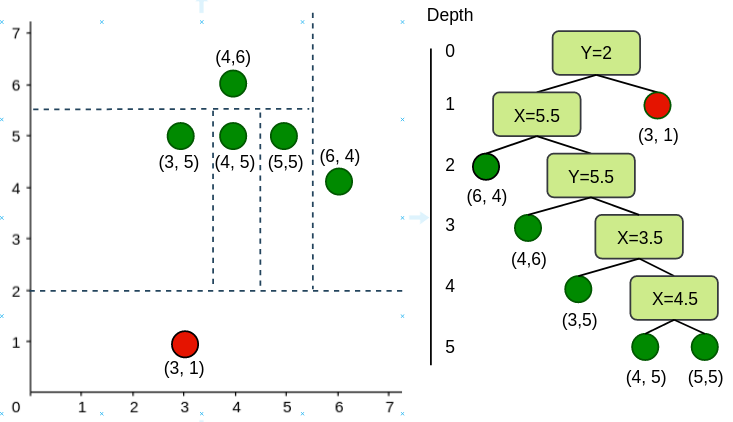
\includegraphics[width=\linewidth]{images/rich_sketch_original.png}
  \caption{}
  \label{fig:rich_sketch_original}
\end{figure}

\section{Methods}\label{sec:methods}
% Notes: 
% Here we describe how the work was done.
% Mathematical description of new model. Maybe pseudocode of algorithm? 
% Discussion of new model? Performance, complexicity, etc? 
% We describe the extended isolation forest here. In Direct Analysis of GD .. the used method has its own section. 
% Concept, and new stuffs
% Running isolation as is directly on bases - phase 1
% Running extended isolation on the bases  - phase 2
% Can include or exclude counts 
% tradeoffs: counts, precision. 

% -----------

% What to include:

\subsection{Isolation Forest on GD compressed Data}
Data compressed with generalized deduplication results in having a set of bases, deviation and references linking a data point to its base and deviation. In the following example the deviation will be omitted. Say we have the data set $S$ where $S \in \mathbb{R}^2$. Performing GD on $S$ will result in each feature of the points being mapped to their bases. Having an point $x = [x_1,x_2]$ where $x \in S$ and some computed bases ids $b_0, b_1, ..., b_n$,then the transformed version $x*=[x^*_1, x^*_2]$ will hold the computed bases. This is depicted on Figure \ref*{fig:gd_points}. The bases are computed on the raw data and referenced in the features $x^*_1$ and $x^*_2$.

\begin{figure}
  \centering
  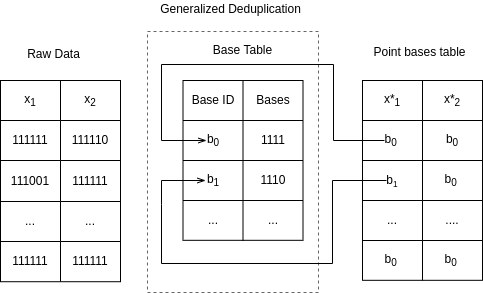
\includegraphics[width=\linewidth]{../files/test.png}
  \caption{}
  \label{fig:gd_points}
\end{figure}

Isolation forest is then to be performed on the transformed version of the data set. The isolation forest splits before compression could be seen on Figure \ref{fig:rich_sketch_original}. Figure \ref{fig:rich_sketch_bases} is similar but is instead performing the splits on the bases. It is seen that certain data points will map to identical bases on both features.  

\begin{figure}
  \centering
  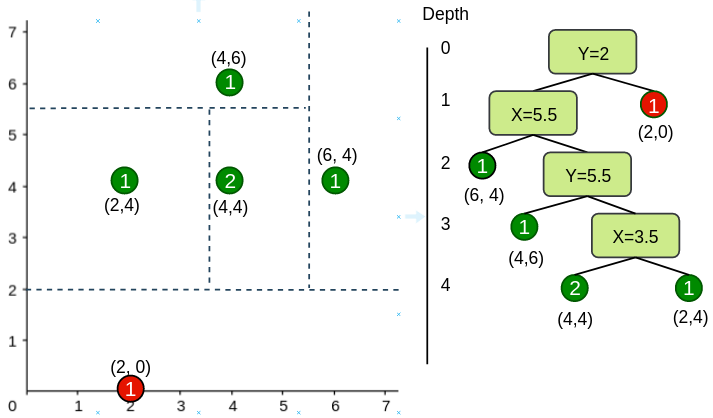
\includegraphics[width=\linewidth]{images/rich_sketch_bases.png}
  \caption{}
  \label{fig:rich_sketch_bases}
\end{figure}


\subsection{DupRes Isolation Forest}
The bases of GD compressed data will inherintly be grouped. Stripping the deviation of each data point will result in data points being placed in bins. This binning is illustrated on figure \ref*{fig:binning}. The graphic shows the bins created with different amount of deviation bits. The circles are the bases. The dotted lines are enclosing areas where data points in an area will be mapped to the closest base in the negative direction. Having a larger amount of deviation bits is leading to larger bins. 

\begin{figure}
  \centering
  \begin{minipage}{0.45\linewidth}
      \centering
      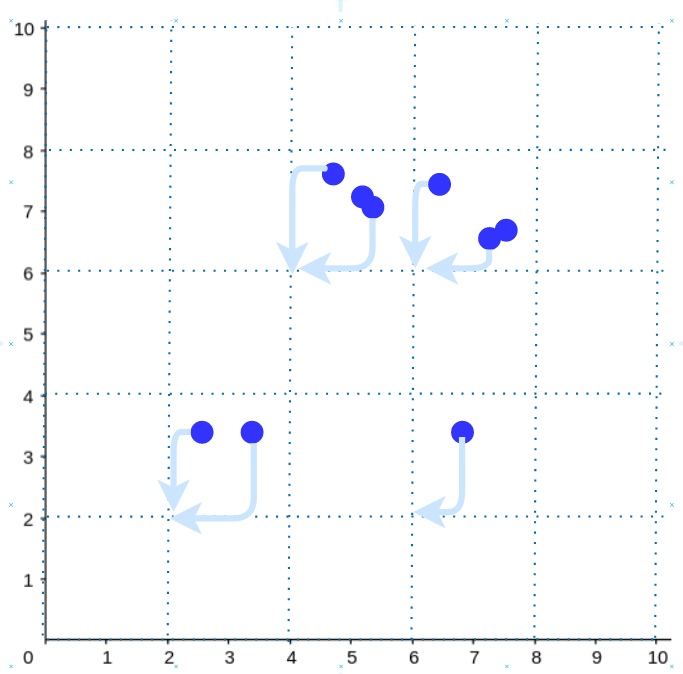
\includegraphics[width=\textwidth]{images/binning-1dev.png}
      \caption{first figure}
  \end{minipage}\hfill
  \begin{minipage}{0.45\linewidth}
      \centering
      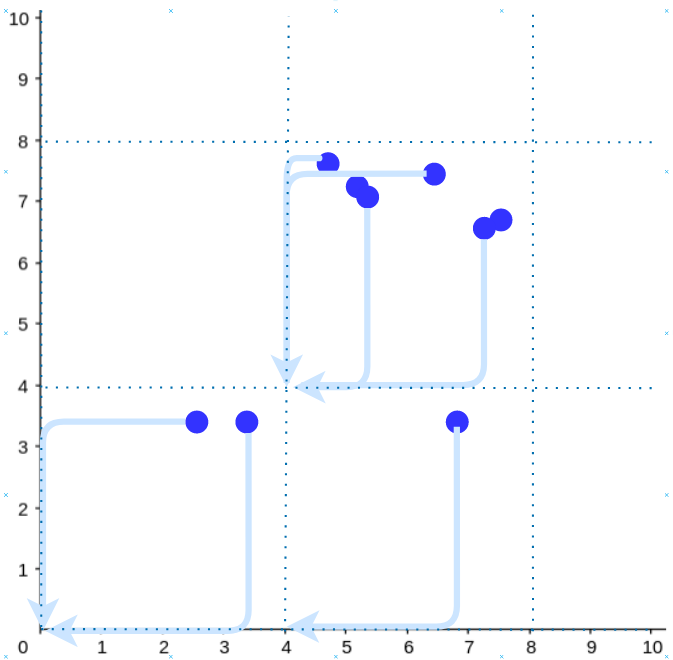
\includegraphics[width=\textwidth]{images/binning-2dev.png}
      \caption{second figure}
  \end{minipage}
\end{figure}

Having larger bins might lead to a better compression rate however it could lead to undesired behaviour when trying to detect anomalies with iForest. An outlier could be mapped to the same base as an inlier on all or some of it features. Having the same base on some features will make it harder to isolate the outlier meanwhile having identical bases on all features makes it impossible. The binning aswell leads to inliers being grouped on fewer points. This causes them to be isolated more easily, and thus labeled as outliers.   

Isolation Forest is not fit for the large amount duplicates that is potentially created by compressing with generalized deduplication. Therefore, a more duplicate resistant (DupRes) version is proposed. The core idea of the new version is to utilize the amount of duplicates when building the tree. The amount is then used to adjust the score of an observation. A revised version of the score function is: 

\begin{equation}
  s(x,n) = 2^{-\frac{E(h(x))+log_2(x_{count})}{c(n)}}
  \label{eq:dupres_score}
\end{equation}     
 
The new function differs from Equation \ref{eq:org_score} by the introduction of the $log_2(x_{count})$ term. $x_{count}$ is the amount of occurences of the given sample. The reason behind using the binary logarithm is firstly that having one occurance will not modify the score, $log_2(1)=0$. Secondly, it is a strictly increasing function. Resulting in the higher the $x_{count}$, the larger adjustments will be made to the score. The modification makes no changes in the range of $s$ and in how it should be interpreted. For further details, see the original paper \cite{iforest}.     

The change implies that the count of each sample is known. This requires extending what is done in the training phase of the model. Beside building the decision trees, the model must store each unique sample with the amount of occurences. Worst case the training set contains no duplicates and will store all training samples with the count of one. Hereby, the model is not optimal if the data is expected to have a low amount of duplicates. The flow during the evaluation of unseen observations, is to identify the ones that was seen in the training phase and retrive their counts. The adjusted score is then computed and can be used to identify anomalies.        

% amount features 
% figure with grouped 
% What is the new method, formulas, tweak log thingy. Training, testing.. 
% - storing all train data in memory :( 
% - how did we derive equations. One more for prins knud. 
% 


\section{Experiments}\label{sec:experiments}
The experimental setup will be described in this section. Three models will be evaluated, Isolation Forest on the original data before compression, Isolation Forest on the compressed data and the proposed DupRes Isolation Forest on the compressed data. We will refer the different model in the same order as, \textbf{original}, \textbf{bases} and \textbf{DupRes}. The models are evaluated on various datasets containing anomalies. The datasets are described in the following subsections.

\subsection*{Synthetic}
The synthetic dataset is self-generated. It is two-dimensional where each feature is an integer. The dataset contains three clusters where the samples are normally distributed with a standard deviation of 2, $N(\mu, 2^2)$ where $\mu$ varies on the cluster center. The data set is represented before and after compression on Figure \ref{fig:synthetic-dataset}. Each cluster consists of 150 samples and 20 outliers are generated between the clusters. There is then a total of 470 samples.

\begin{figure}
  \centering
  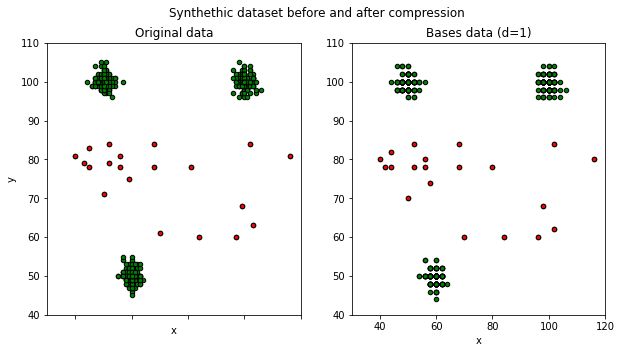
\includegraphics[width=\linewidth]{images/synthethic-dataset.png}
  \caption{Synthetic data set before(left) and after(right) compression with 1 deviation bit. Green points are inliers, while the red are outliers. }
  \label{fig:synthetic-dataset}
\end{figure}

\subsection*{Pendigits}
Pendigts is a database for handwritten digits. Originally it contains 16 integer features  with 10 classes (one for each digit). The dataset's 6870 samples is mapped to inliers and outliers to be utilized for anomaly detection \cite{ODDS}.

\subsection*{Shuttle}
The shuttle dataset contains 49097 samples collected from a shuttle. It has 9 dimensions all being integers \cite{ODDS}.

\subsection*{Waveform}
Waveform contains 3443 samples with 100 outliers. It has 21 features that are all numeric \cite{waveform}.

\subsection*{WBC}
The WBC dataset contains data of measurements from breast cancer cases. The inliers are the benign class, while the outliers are the malignant class. It contains 278 samples with 30 dimensions \cite{ODDS}.

\subsection{Preprocessing}
All the features of the synthetic, pendigits and shuttle datasets can be represented as a one byte integer. However, the WBC and waveform datasets contains floating numbers. Therefore, the features are scaled with a factor of 10.

\subsection{Procedure}
The experiments are realized in Python and can be found for replication on GitHub\footnote{\href{https://github.com/mlRosenquist/au-mlr-research-and-development-dedup}{https://github.com/mlRosenquist/au-mlr-research-and-development-dedup}}. DupRes is implemented by extending \textit{sklearn}'s existing Isolation Forest functionality. Thus, a fork is as well to be found on GitHub\footnote{\href{https://github.com/mlRosenquist/scikit-learn}{https://github.com/mlRosenquist/scikit-learn}}.
Each dataset is split in a training set and test set with a 80\%/20\% proportionality. The split is done in a stratified manner, meaning it is ensured to be inliers and outliers in both sets. We had the three models; \textbf{original}, \textbf{bases} and \textbf{DupRes}. The original requires no additional transformation of the data. However, the other two requires the GD compressed version of the data. Hence, we store both the original and the compressed data. The models are then trained on the training data and evaluated on the test data in sequence.

\subsection{Performance evaluation}
As Isolation Forest by nature introduces randomness in building its decision trees, we train and evaluate each model 50 times. At each iteration various performance metrics are stored. When all iterations are complete we remove the lowest and highest scoring of each metric and take the mean of the remaining values. The mean value is then the resulting value for that metric on a given model. The different metrics that is looked at is training time, testing time, accuracy, f1, recall and precision. The training and testing time tells, how much processing time is used to fit the model on the training data and to predict unseen samples in form of the test data. Accuracy show in percentage how many observations are predicted correctly. Recall relate to the ability of finding all positive samples. In the experiments conducted we have set the inliers to be the positives while the outliers to be the negatives. Precision includes the false positives in its calculation. This means in our case that precision can intuitively be used to see if the outliers are correctly detected. The f1-score is the harmonic mean of the precision and recall \cite{sklearn}.





\section{Results}\label{sec:results}
\unfinished{write results}

% Notes: 

% -----------

% What to include:

\begin{figure}
  \centering
  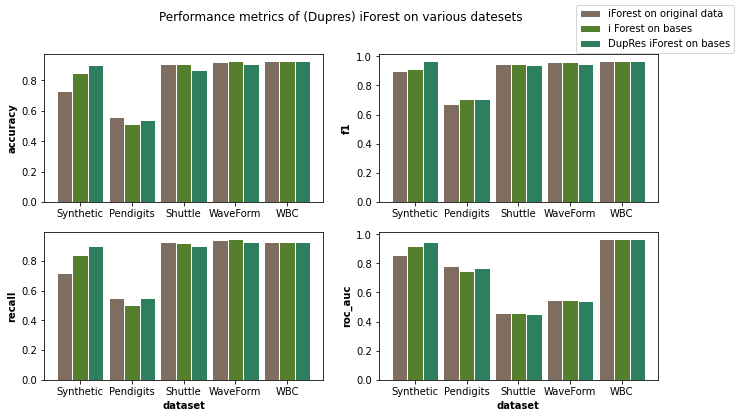
\includegraphics[width=\linewidth]{images/performance_metrics.png}
  \caption{}
  \label{fig:performance_metrics}
\end{figure}

\begin{figure}
  \centering
  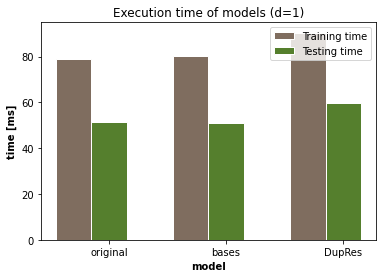
\includegraphics[width=0.8\linewidth]{images/performance_time.png}
  \caption{}
  \label{fig:performance_time}
\end{figure}

\section{Conclusion}\label{sec:conclusion}
This paper looked into performing anomaly detection on compressed data. Generalized deduplication was the compression algorithm of choise, that enables direct analysis of the bases derived from the transformed data. The amount of compression controlled the clustering and performance of the anomaly detection models. The duplicates created by the algorithm is taken advantage of in an extended version of Isolation Forest. Comparing the proposed model with original Isolation Forest it showed that utilizing the duplicates improves classification performance. However, the improved scoring is a tradeoff with memory usage and execution time. A general observation is that performing Isolation Forest on the uncompressed data versus compressed had no large descrepancies in performance.    

\section{Future work}
DupRes currently uses the $log_2(x_{count})$ term to tune the score towards being an inlier based on the count. This is potentially a hyperparameter that can be tuned. Maybe a completely different term fits better. This could be something that also includes the dimensionality of the data or other factors. This report looked at a limited amount of datasets. It would therefore be interesting to see how the different models perform on others. In regards to generalized deduplication we only investigated 8 bit integers. Thus, a task is to research the anomaly detection behaviour on floating numbers.      

\printbibliography[title={References}]

\end{document}